\chapter{Stars, Bars and Hockey Sticks}
While most problems can be solved using the basic methods, sometimes its better to 
remember a certain fact. This chapter covers some common equivalence as well as some 
common combinatorial sums. We will start with Stars and Bars or Beggar's Theorem which 
is one of the most famous equivalences ever.
\section{Stars and Bars}
\begin{example}
    [Motivating Example] In how many ways can $10$ chocolates be divided 
    among $3$ children(The children are distinguishable, the chocolates aren't)?
\end{example}
\begin{proof}
    [Solution]
    This question is basically number of ordered tuples $(a,b,c)$ such 
    that $a+b+c=10$ given that $a,b,c \geq 0$.\par
This means we can re frame the question as ways to insert two 
identical bars among ten identical stars. Note that this is equivalent 
as the stars will be divided into three parts which will sum to $10$. As the 
problem is same, so is the solution, hence:\par
We are looking for the permutations of this configuration which will be: 
$\frac{(10+2)!}{2!*10!}$ Which is equal to $66$.
\end{proof}
Note that it is also possible to get the solution with casework in this 
particular question. However, doing so will become increasingly impractical 
as the number of children and chocolates will increase.\par 
We can generalize the above idea as:
\begin{theorem}
[Stars and Bars]
    we can say the number ways to put $n$ similar objects in $k$ distinguishable bins 
    is equivalent to permuting $n$ stars and $k-1$ bars which is equal 
    to $\frac{(n+k-1)!}{n!*(k-1)!}=\binom{n+k-1}{n}$
\end{theorem}
The Stars and Bars has various uses. The vanilla use of it comes up 
routinely in collage entrances. It can be made a little more spicy by doing a small change.
\begin{example}
    Alice has $24$ apples. In how many ways can she share them with Becky and 
    Chris so that each of the three people has at least two apples?
\end{example}
\begin{proof}
    [Solution]
    As everyone needs to have $2$ apples, let's start by giving everyone $2$ apples 
    to begin with. This means we have to divide $18$ apples with $3$ people. This is 
    the classical stars and bars. So the answer is $\binom{20}{2}$.
\end{proof}
This question can be boosted a bit more if every apple limit? For 
example let's say Alice must have at least $3$ apples, Becky at least $2$ and Chris 
at least $1$. The solving(and in this case the answer) remains the same.\par
We can get it a bit more spicy.
\begin{example}
    Find the number of positive integer quadruples $(a, b, c, d)$ that satisfy $a+b+c+d<24$.
\end{example}
\begin{proof}
    [Solution]
    Let $a+b+c+d=24-e \iff a+b+c+d+e=24$ where $e$ is a positive integer. 
    This means $a,b,c,d,e$ are all positive integers. Note that $0$ is neither 
    positive nor negative. So all of them are at least $1$.\par
    This means we are back to a Stars and Bars problem. Give all of them $1$ to start with 
    and then inserting in the theorem we get $\binom{23}{4}$.
\end{proof}
To lead us to the next part, I'll need you to notice something:\par
We could use casework on this question. So we want to solve $a+b+c+d=k$ for $k=3,\dots,23$. Using 
Stars and bars, we get the solution to each of the case by giving $a,b,c,d$ $1$ each to begin 
with. So using stars and bars, $\binom{k-4+3}{3}=\binom{k-1}{3}$ for some value of $k$. 
This means $\binom{3}{3}+\dots+\binom{22}{3}$ is the answer.\par
We already know the answer is $\binom{23}{4}$ and as they are equal, 
we get: $\binom{3}{3}+\dots+\binom{22}{3} = \binom{23}{4}$\par
\section{Counting in two ways}
Let's talk about a last chapters once. While playing the guessing game, 
you may have found yourself having two or more ways to solve the same question both, 
hopefully, leading to the same answer. But as one method is easier to compute than the 
other, we should use that. But that doesn't prevent us from thinking about it.\par
Given a configuration, we should get the same answer from any which methods. This 
means we can count in two ways.\par
This idea is what we use to create some combinatorial identities. We calculate the 
same thing generalized thing in two ways and equate them to get an identity, which 
we can use elsewhere as it is true in general.\par
This is called counting in two ways. Let's see it in action:
\begin{example}
    [Motivating Example]
    How many councils with at least $1$ member and at most $n$ members be made 
    from a pool of $n$ people?
\end{example}
\begin{proof}
    [Solution]
    We obviously know that the answer is $2^n - 1$ from the subset theorem. \par
    However we can also write this as $\binom{n}{1} + \binom{n}{2} \dots \binom{n}{n}$\par
    We can, hence say, $\binom{n}{1} + \binom{n}{2} \dots \binom{n}{n}= 2^n -1$ \par
    $\therefore \binom{n}{1} + \binom{n}{2} \dots \binom{n}{n} +1 = 2^n$ \par
    as we know $\binom{n}{0}=1$, we can say: $\binom{n}{0} + \binom{n}{1} + \binom{n}{2} 
    \dots \binom{n}{n} = 2^n$
\end{proof}
What we just derived is called the Binomial identity.
\begin{theorem}
    $\binom{n}{0} + \binom{n}{1} + \binom{n}{2} \dots \binom{n}{n} = 2^n$
\end{theorem}
Let's talk about the name of the identity for a while.\par
Binomial in math refers to polynomial with $2$ terms. For example $x+2$ or $3x+7$, in general $ax+b$.\par
If you have already studied some algebras, you may know that $(a+b)^2=a^2+2ab+b^2$ 
and $(a+b)^3=a^3+3a^2b+3ab^2+b^3$. These are normally derived by opening the brackets and multiplying(FOIL).\par
But how do we find $(a+b)^4$ or worse $(a+b)^{10}$. \par
We can notice that all the terms of the expansion of $(a+b)^k$ are $a^mb^n$ where $m+n=k$. 
I smell some combinatorics...\par
\begin{theorem}
    [Binomial Theorem]
    \[(a+b)^n = \binom{n}{0}a^{n}b^0+\binom{n}{1}a^{n-1}b^1+\dots+
    \binom{n}{n-1}a^{1}b^{n-1}+\binom{n}{n}a^{0}b^{n} = 
    \sum_{m=0}^{k}{\binom{k}{m}}\cdot a^m\cdot b^{k-m}\]
\end{theorem}
\begin{proof}
    As expected, The Binomial Theorem has a nice combinatorial proof:\par
We can write $(a+b)^k=\underbrace{ (a+b)\cdot(a+b)\cdot(a+b)\cdot\cdots\cdot(a+b) }_{k}$. 
Repeatedly using the distributive property, we see that for a term $a^m b^{k-m}$, we must 
choose $m$ of the $k$ terms to contribute an $a$ to the term, and then each of the other $k-m$ terms 
of the product must contribute a $b$. Thus, the coefficient of $a^m b^{k-m}$ is the number of ways to 
choose $m$ objects from objects $k$, or $\binom{k}{m}$. Extending this to all possible values of $m$ 
from $0$ to $k$, we see that $(a+b)^k = \sum_{m=0}^{k}{\binom{k}{m}}\cdot a^m\cdot b^{k-m}$, as claimed.
\end{proof}
This is also the reason $\binom{n}{k}$ is called a binomial coefficient.\par
Why is the binomial theorem useful here? We can use the binomial theorem to 
expand $(1+1)^n=\binom{n}{0}+\binom{n}{1}+\dots+\binom{n}{n-1}+\binom{n}{n}=2^n$\par
There a lot more uses of binomial theorem as well. Unfortunately, we shall not cover them in this book.\par
Let's look at some more identities.\par
\begin{example}
    [Motivating Example]
     Suppose a committee consists of $m$ men and $n$ women. In how many ways can a 
     subcommittee of $r$ members be formed?
\end{example}
\begin{proof}
    [Solution]
    We obviously know that the answer is $\binom{m+n}{r}$. \par
    However we can also do some case work. Let's say a committee has $0$ men 
    and $r$ women. Then $1$ man and $r-1$ women. And so on. We can write 
    this as $\binom{m}{0}*\binom{n}{r-0} + \binom{m}{1}*\binom{n}{r-1} 
    \dots +\binom{m}{r-1}*\binom{n}{1}+\binom{m}{r}*\binom{n}{0}$\par
    We can, hence say, 
    \[\binom{m}{0}*\binom{n}{r-0} + \binom{m}{1}*\binom{n}{r-1} 
    \dots +\binom{m}{r-1}*\binom{n}{1}+\binom{m}{r}*\binom{n}{0}=\binom{m+n}{r}\]
    \end{proof}
This is called Vandermonde’s Identity.
\begin{theorem}
    $\binom{m}{0}*\binom{n}{r-0} + \binom{m}{1}*\binom{n}{r-1} \dots +
    \binom{m}{r-1}*\binom{n}{1}+\binom{m}{r}*\binom{n}{0}=\binom{m+n}{r}$
\end{theorem}
\section{Pascal's Triangle}
\begin{figure}
    \centering
    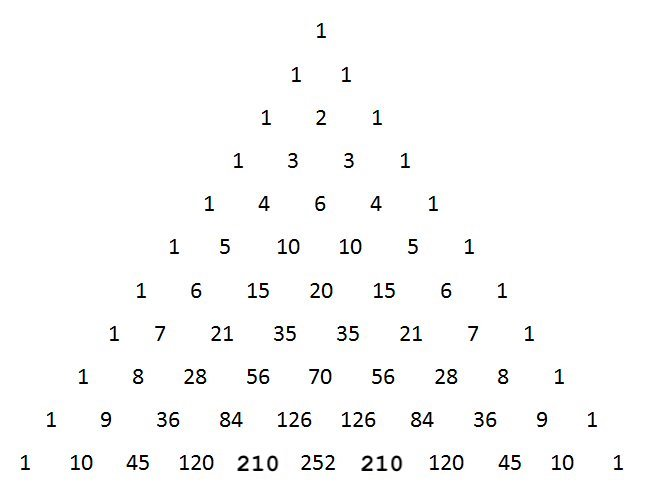
\includegraphics[width=0.75\linewidth]{Photos/Pascal's Triangle.png}
    \caption{Pascal's Triangle: A wonder of the mathematical world}    
\end{figure}
The triangle somewhere on the top of the page is called Pascal's triangle. \par
It has a lot of fun and amazing properties(try to find them, you'll be surprised).\par
We are going to exploit two of them right now. First being, Every term in 
subsequent line is made by adding the two above it. As it turned out, every ancient 
civilization did reach this triangle by doing just that. The second one, the reason 
Blaise Pascal gets to have his name on it.
\begin{figure}
    \centering
    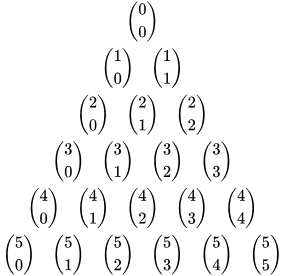
\includegraphics[width=0.75\linewidth]{Photos/Binomial Pascal}
    \caption{As it turns out, we can write everything as a binomial coefficient here.}
\end{figure}
This is exceptionally useful as this leads us to Pascal's Identity....
\begin{theorem}
    $\binom{n}{k} + \binom{n}{k+1}=\binom{n+1}{k+1}$
\end{theorem}
Remember, we saw this while proving principle of inclusion exclusion. 
There we proved it algebraically. We also 'proved' it in a sort of hand wavy manner 
above using pascal's triangle. Here is an another proof, combinatorial this time, for it.
\begin{proof}
    Let's consider choosing a team of $k$ lawyers from a pool of $n-1$ junior lawyers and $1$ Harvey Specter.\par
    The answer is $\binom{n}{k}$. Using casework, We can either have Harvey on the 
    team or not on it. If Harvey is on the team, we have $\binom{n-1}{k-1}$ ways to 
    choose rest of the lawyers. If we don't have Harvey on it, we have $\binom{n-1}{k}$ ways to 
    choose the team.\par
    This means $\binom{n-1}{k-1}+\binom{n-1}{k}=\binom{n}{k}$.
\end{proof}
Finally, here is the hockey stick identity(try looking at a diagonal 
in the triangle, that's where the name comes from). We started this 
section at this identity, and I'll let you prove it.
\begin{theorem}
    $\binom{k}{k}+\binom{k+1}{k}+ \dots +\binom{n}{k}=\binom{n+1}{k+1}$
\end{theorem}
Now here is the first thing, you should remember these identities. They can be memorized 
quite simply by writing them on a piece of paper and taping them to a wall next to where 
you sleep. Every morning look at it just after you wake up, and every night just before you 
sleep. You'll have them memorized in less then a week.\par
The another way to remember(the one which I remember), is by simply solving the questions and 
deriving every identity you forget, no turning the pages back. That will get it done in less 
than two hours flat.
\section{Exercises}
Solve at least questions worth \points{60}. This exercise has a total of \points{75}.
\begin{xcb}{Exercises}
\begin{enumerate}
\item \points{2} In how many ways can one get $10$ upon rolling $7$ dice?
\item \points{2} How many $4$ digit numbers have a sum of $9$?
\item \points{3} How many ordered pairs $(a,b,c,d)$ where $a \le b \le c \le d \le 5$ and $a,b,c,d \in \mathbb{N}$?
\begin{hint}
    \addhint{Let $a=1+x$, $b=a+y$ and so on. Does this look like a Stars and Bars now?}
\end{hint}
\item (AIME 2000) \points{9} Given that\par
\[\frac 1{2!17!}+\frac 1{3!16!}+\frac 1{4!15!}+\frac 1{5!14!}+\frac 1{6!13!}+\frac 1{7!12!}+\frac 1{8!11!}+\frac 1{9!10!}=\frac N{1!18!}\]
find the greatest integer that is less than $\frac N{100}$.
\begin{hint}
    \addhint{Multiply both sides by $19!$}\par
    \addhint{Multiply both sides by $2$ and use $\binom{n}{k}=\binom{n}{n-k}$}
    \addhint{Add terms to reach an identity which we know the summation to}
\end{hint}
\item(AIME 2001) \points{3} A fair die is rolled four times. The probability that each of the final three rolls is at least as large as the roll preceding it may be expressed in the form $m/n$ where m and n are relatively prime positive integers. Find $m + n$.
\item (AMC 8 2018) \points{3} From a regular octagon, a triangle is formed by connecting three randomly chosen vertices of the octagon. What is the probability that at least one of the sides of the triangle is also a side of the octagon?
\begin{hint}
    \addhint{Can we convert the choosing of $3$ points as partitioning of remaining $5$ points into $3$?}
\end{hint}
\item(AIME 2020) \points{2} A club consisting of $11$ men and $12$ women needs to choose a committee from among its members so that the number of women on the committee is one more than the number of men on the committee. The committee could have as few as $1$ member or as many as $23$ members. Let $N$ be the number of such committees that can be formed. If $N=\binom{a}{b}$, find $a + b$
\begin{hint}
    \addhint{We'll use Vandermonde identity, now try to solve it.}
\end{hint}
\item (AIME 2015) \points{3} Consider all 1000-element subsets of the set ${{1, 2, 3, \dots , 2015}}$. From each such subset choose the least element. The arithmetic mean of all of these least elements is $p/q$, where $p$ and $q$ are relatively prime positive integers. Find $p + q$.
\begin{hint}
    \addhint{$a_1+2a_2+3a_3+\dots na_n=(a_1+a_2+\dots+a_n)+(a_2+a_3+\dots)+\dots+(a_n)$}
\end{hint}
\item \points{2} For how many positive integers $x_1, x_2, \dots, x_{10}$ do we have $x_1 + x_2 + \dots + x_{10} = 50$?
\item (AIME 2011) \points{5} Ed has five identical green marbles, and a large supply of identical red marbles. He arranges the green marbles and some of the red ones in a row and finds that the number of marbles whose right hand neighbor is the same color as themselves is equal to the number of marbles whose right hand neighbor is the other color. An example of such an arrangement is $GGRRRGGRG$. Let $m$ be the maximum number of red marbles for which such an arrangement is possible, and let $N$ be the number of ways he can arrange the $m+5$ marbles to satisfy the requirement. Find the remainder when $N$ is divided by $1000$.
\begin{hint}
    \addhint{$m$ is limited by the fact that number of marbles whose right hand neighbor is the other color is maximum 10. How many red marbles will we need for this to lead to a valid arrangement?}
    \addhint{As we know $m$ now, can we simply use stars and bars with one red marble always between 2 green.}
\end{hint}
\item (AIME 2011) \points{9} Six men and some number of women stand in a line in random order. Let $p$ be the probability that a group of at least four men stand together in the line, given that every man stands next to at least one other man. Find the least number of women in the line such that $p$ does not exceed 1 percent.
\begin{hint}
    \addhint{In what ways can the men be arranged in? Use the groups of men as bars and the women as stars}
    \addhint{Use Pascal to simplify and then open the binomial}
\end{hint}
\item \points{2} Let $n$ be a positive integer. In how many ways can one write a sum of at least two positive integers that add up to $n$?
\item (AIME 2013) \points{5} Melinda has three empty boxes and $12$ textbooks, three of which are mathematics textbooks. One box will hold any three of her textbooks, one will hold any four of her textbooks, and one will hold any five of her textbooks. If Melinda packs her textbooks into these boxes in random order, the probability that all three mathematics textbooks end up in the same box can be written as $\frac{m}{n}$, where $m$ and $n$ are relatively prime positive integers. Find $m+n$.
\begin{hint}
    \addhint{Casework onto the box in which the three math textbooks are in}
    \addhint{Simplify before you compute! Take $9!$ common, multiply numerator and denominator by $3!4!5!$}
\end{hint}
\item (AMC 10 2016) \points{3} For some particular value of $N$, when $(a + b + c + d + 1)^N$ is expanded and like terms are combined, the resulting expression contains exactly $1001$ terms that include all four variables $a, b, c,$ and $d$, each to some positive power. What is $N$?
\item (AMC 12 2021) \points{9} A choir director must select a group of singers from among his $6$ tenors and $8$ basses. The only requirements are that the difference between the number of tenors and basses must be a multiple of $4$, and the group must have at least one singer. Let $N$ be the number of different groups that could be selected. What is the remainder when $N$ is divided by $100$?
\begin{hint}
    \addhint{Casework on the tenors $-$ basses combined with Vandermonde will work.}
\end{hint}
\item (IMO 1981/2) \points{9} Let $\displaystyle 1 \le r \le n$ and consider all subsets of $\displaystyle r$ elements of the set $\{ 1, 2, \ldots , n \}$. Each of these subsets has a smallest member. Let $\displaystyle F(n,r)$ denote the arithmetic mean of these smallest numbers; prove that\par
\[F(n,r) = \frac{n+1}{r+1}.\]
\begin{hint}
    \addhint{We have already solved a case of it as an AIME 2015 problem, won't the same technique work in general?}
\end{hint}
\item \points{5} Prove that \[\sum_{k=0}^n k{\binom{n}{k}}^2=n\binom{2n-1}{n-1}\]
\item Given a positive integer $n$, what is the largest $k$ such that the numbers $1, 2, \dots , n$ can be put
into $k$ boxes such that the sum of the numbers in each box is the same?
\end{enumerate}
\end{xcb}